%  A description of the observer and the implemented controller including a schematic.
Controller technology in control engineering is about the design and implementation of structures that regulate the behavior of a dynamic systems. Controllers are needed to maintain desired system outputs by adjusting system inputs usually based on feedback signals. Advanced controller technologies like an observer, specifically a state observer or an observer-based controller, is a component used in control systems to estimate the state variables of a system based on its inputs and outputs. It does not directly influence the control action but provides valuable information for feedback control.

For this laboratory the control structure was given by the lecturer to achieve proper results. In figure \ref{fig:controlStruct} one can see the whole structure with the controller and the observer in gray rectangles as well as the system in state space representation.

\FloatBarrier
\begin{figure}[ht]
	\begin{center}
        % trim = left bottom right top
		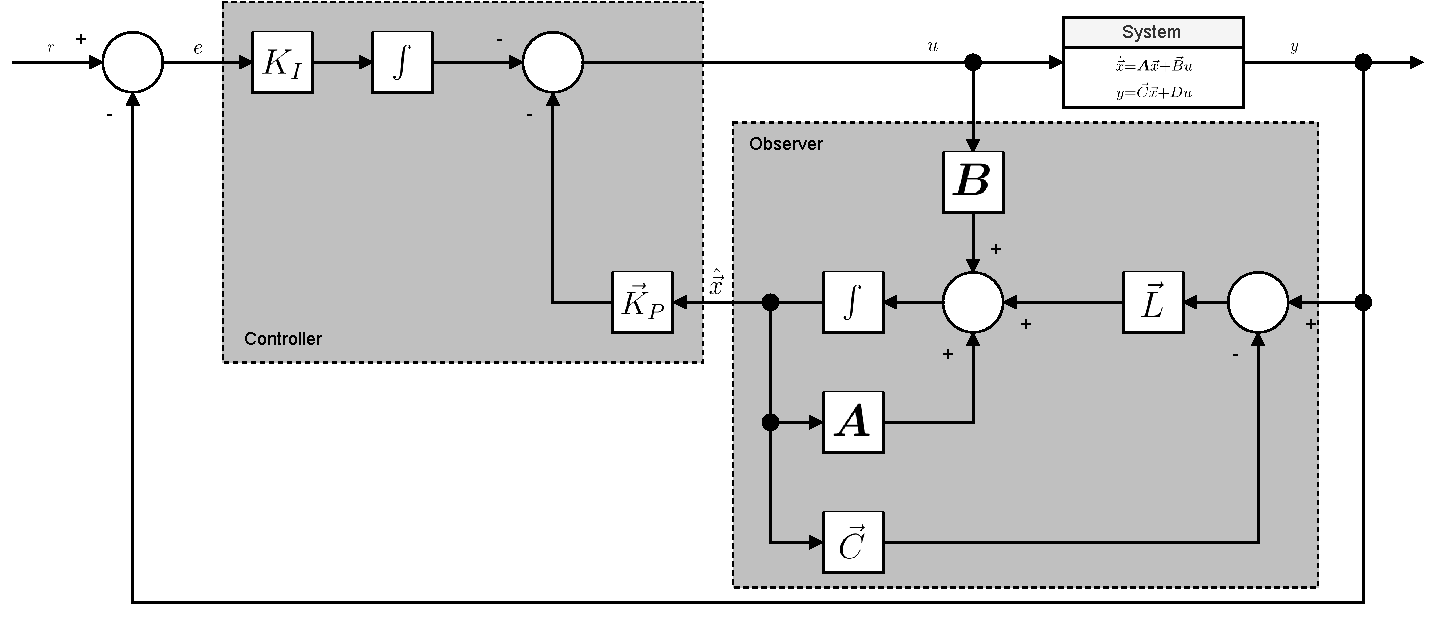
\includegraphics[clip, trim=0cm 0cm 0cm 0cm, width=0.7\textwidth]{figure/controllerTechnology.pdf}
		\caption[Control structure]{Control structure}
		\label{fig:controlStruct}
	\end{center}
\end{figure}
\FloatBarrier

The control architecture is based on the feedback of the system output $y$ as well as the system states $\hat{\Vec{x}}$, which are estimated by the observer. At the sum of the controller block, both the $K_i$ and the $K_p$ signal are substracted. This leads to a higher stability of the control structure because of a higher damping. The used observer technology is called a \textit{Luenberger Observer} which will be described in more detail in chapter \ref{subsec:observer}.

\subsection{Controller} \label{sec:controller}
For the state feedback control the two parameters settling time $t_s = \SI{4}{s}$ and the percentage overshoot $PO = 5\,$ are chosen. With equation \ref{eqn:zeta} and \ref{eqn:naturalw} the damping ratio $\zeta = 0.69$ and the natural frequency $\omega_n = 1.45$ can be defined.
\begin{equation}
    \zeta = \sqrt{\frac{\log(PO)^2}{\pi^2 + \log(PO)^2}}
    \label{eqn:zeta}
\end{equation}
\begin{equation}
    \omega_n = \frac{4}{\zeta * t_s}
    \label{eqn:naturalw}
\end{equation}
With $\zeta$ and $\omega_n$ two complex conjugated poles can be calculated with $p_2 = -1.00 + 1.05i$ and $p_3 = -1.00 - 1.05i$. The first one will be not so dominant and therefore more left $p_1 = p_2 \cdot 2 = -2.00 + 2.10i$. Because of no permanent control error due to a step input we get two new matrices like in equation \ref{eqn:ABstrich}. \cite{Skript}
\begin{equation}
\begin{split}
    A' &= \begin{bmatrix} 0 & 0 & -1.57 \cr 0 & -2.20 & -1.57 \cr 0 & 1 & 0 \end{bmatrix} \\
    B' &= \begin{bmatrix} 0 \cr 1 \cr 0 \end{bmatrix} 
    \label{eqn:ABstrich}
\end{split}
\end{equation}
The control parameters $K_i = -3.67$ and $K_p = \begin{bmatrix} 1.80 & 4.53 \end{bmatrix}$ are then calculated by pole placement method place($A', B', \begin{bmatrix} p_1 & p_2 & p_3 \end{bmatrix}$) in MATLAB. 

\subsection{Observer} \label{subsec:observer}
The Luenberger observer estimates the state(s) of the system. It may contain the controlled variable, the derivative of the controlled variable or other internal variables of the system. To achive this the Luenberger observer uses a model of the real system to create an estimation. In our case the observer uses the measurement of the controlled system output $y$ and the control signal $u$ to estimate the state of the system. To design a proper Luenberger observe we simply define two poles at $p_1 = -4$ and $p_2 = -6$. Afterwards with the transposed system matrix $\boldsymbol{A}'$ and output matrix $\boldsymbol{C}'$ the \textit{place} method in MATLAB creates the observe gain matrix $\boldsymbol{L} = place(\boldsymbol{A}',\boldsymbol{C}',\begin{bmatrix} p_1 & p_2 \end{bmatrix})$ whicht leads to equation \ref{eqn:obsGain}.
\begin{equation}
    \boldsymbol{L} = \begin{bmatrix} 3.36 \cr 4.96 \end{bmatrix} 
    \label{eqn:obsGain}
\end{equation}